\chapter{Linear Methods for Regression}
%% TODO LIST
% LAR REGRESSION
% MULTIPLE OUTCOME SHRINKAGE AND SELECTION
% More on the Lasso and Related Path Algorithms

Useful in situations with small numbers of training cases, low signal-to-noise ratio, 
or sparse data. 
\section{Linear Regression Models and Least Squares}
Consider linear model
\begin{equation*}
	f(X)=\beta_0+\sum_{j=1}^{p}X_j\beta_j
\end{equation*}
which assume the regression function $E(Y|X)$ linear or the linear model is a good 
approximation. 
Here $X_j$ can be
\begin{itemize}
	\item Quantitative inputs
	\item Transformation/Basis expansion of inputs e.g. log, square-root, polynomial
	\item Numeric/dummy coding of the levels of the inputs
\end{itemize}
\begin{equation*}
	RSS(\beta)=(y-X\beta)^T(y-X\beta)
\end{equation*}
$X$ has full column rank$\Rightarrow X^TX$ positive definite. 

By solution, we have $\hat{y}=X\beta=X(X^TX)^{-1}X^TY, \hat{y_i}=x_i^T\hat{\beta}$
\begin{itemize}
    \item $H=X(X^TX)^{-1}X^T$: hat matrix, which computes the orthogonal projection 
    from $Y$ to $\hat{Y}$. 
\end{itemize}

When columns of $X$ are not independent
\begin{itemize}
    \item Perfectly correlated$\Rightarrow X^TX$ singular, $\hat{\beta}$ not uniquely 
    defined. However, $\hat{y}$ are still the projection from $y$ to column space of 
    $X$. 
	\begin{itemize}
        \item May appear when number of inputs $p$ exceed the number of training cases $N$, 
        where features reduced by filtering or fitting controlled by regularization. 
	\end{itemize}
\end{itemize}

If $y_i$ are uncorrelated with constant variance $\sigma^2$ and $x_i$ are fixed
(non random), then we have estimation
\begin{align*}
Var(\hat{\beta})=&E[(\hat{\beta}-\beta)(\hat{\beta}-\beta)^T]
=E[((X^TX)^{-1}X^T\epsilon)((X^TX)^{-1}X^T\epsilon)^T]=(X^TX)^{-1}\sigma^2\\
\hat{\sigma}^2=&\frac{1}{N-p-1}\sum\limits_{i=1}^N(y_i-\hat{y_i})^2
\end{align*} 
where $N-p-1$ makes $\hat{\sigma^2}$ is an unbiased estimation because 
$\sum\limits_{i=1}^N(y_i-\hat{y_i})^2\sim \sigma^2\chi^2_{N-p-1}$. 

Now we assume the linearity of the model and deviations of $Y$ around its expectation 
are additive and Gaussian,  consider the model
\begin{equation*}
Y=E(Y|X_1,...,X_p)+\epsilon=\beta_0+\sum\limits_{j=1}^pX_j\beta_j+\epsilon
\end{equation*}
where $\epsilon\sim N(0,\sigma^2)$, 
then $\hat{\beta}\sim N(\beta,(X^TX)^{-1}\sigma^2), 
(N-p-1)\hat{\sigma}^2\sim \sigma^2\chi_{N-p-1}^2$, and $\hat{\beta},\hat{\sigma}^2$ 
statistically independent. 

~

To test \textbf{whether $\beta_j=0$}, we consider Z-score
\begin{equation*}
	z_j=\frac{\hat{\beta}_j}{\hat{\sigma}\sqrt{v_j}}
\end{equation*}
where $v_j$ is the $j$th diagonal element of $(X^TX)^{-1}$, under null hypothesis, 
$z_j$ is distributed as $t_{N-p-1}$, thus a large value of $z_j$ will reject the null 
hypothesis. 
\begin{itemize}
	\item When $\hat{\sigma}$ is replaced by $\sigma$, $z_j$ is normally distributed. 
	\item Difference of tail quantiles will be small when sample size increases. 
\end{itemize}

~

To test the \textbf{significance of groups of coefficients}, e.g. whether a variable 
can be excluded, we need to test whether its coefficients can all be set to zero, 
here we use F-statistics
\begin{equation*}
F=\frac{(RSS_0-RSS_1)/(p_1-p_0)}{RSS_1/(N-p_1-1)}
\end{equation*}
where $RSS_1$ is the residual sum of squares with $p_1+1$ parameters, $RSS_0$ for 
the nested smaller model with $p_0+1$ parameters, having $p_1-p_0$ constrained to 
be $0$, F statistics measures the change in residual sum of squares per additional 
parameter in the bigger model. 

Under Gaussian assumption and null hypothesis that smaller model is correct, 
$F\sim F_{p_1-p_0,N-p_1-1}$. 
\begin{itemize}
	\item $z_j$ is equivalent to F statistics when only drop one coefficient. 
    \item When $N$ is large enough, quantiles of $F_{p_1-p_0,N-p_1-1}$ approach those 
    of the $\chi^2_{p_1-p_0}$
\end{itemize}

When we can isolate $\beta_j$ to obtain a $1-2\alpha$ confidence interval for 
$\beta_j$
\begin{equation*}
    (\hat{\beta}_j-z^{(1-\alpha)}v_j^{\frac{1}{2}}\hat{\sigma}, 
    \hat{\beta}_j+z^{(1-\alpha)}v_j^{\frac{1}{2}}\hat{\sigma})
\end{equation*}
where $z^{(1-\alpha)}$ is the $1-\alpha$ percentile of normal distribution. 

We can also obtain an approximate confidence set for the entire parameter vector 
$\beta$
\begin{equation*}
    C_{\beta}=\{\beta|(\hat{\beta}-\beta)^T(\hat{\beta}-\beta)\le\hat{\sigma}^2 
    {\chi^2_{p+1}}^{(1-\alpha)} \}
\end{equation*}
This confidence set for $\beta$ generates a corresponding confidence set for 
$f(x)=x^T\beta$, namely $\{x^T\beta|\beta\in C_{\beta}\}$

~

Another way of comparing significance between different variables: Use 
Z-score=mean/std of coefficient and compare Z-score of different variables. 
Z-score$>2$ implies significance at 5\% level

\subsection{The Gauss-Markov Theorem}
\begin{itemize}
    \item Least squares estimates of $\beta$ have the smallest variance among all 
    linear unbiased estimates. 
	\item Unbiased estimation may not be a wise choice. 
\end{itemize}

Consider linear combination of parameters $\theta=a^T\beta$, then the least square 
estimates of $a^T\beta$ is
\begin{align*}
	\hat{\theta}=&a^T\hat{\beta}=a^T(X^TX)^{-1}X^TY\\
    E(a^T\hat{\beta})=&E(a^T(X^TX)^{-1}X^Ty)=
    a^T(X^TX)^{-1}X^TE(y)=a^T(X^TX)^{-1}X^TX\beta=a^T\beta
\end{align*}
Thus $a^T\hat{\beta}$ is unbiased if the linear model is correct. 

\begin{thm}
    (Gauss-Markov theorem) If we have any other unbiased linear estimator 
    $\tilde{\theta}=c^Ty$ for $a^T\beta$, then $Var(a^T\hat{\beta})\le Var(c^Ty)$
\end{thm}
\begin{proof}
	Triangle inequality. 
\end{proof}
\begin{rem}
	Can be extended to entire parameter $\beta$ with a few more definition. 
\end{rem}

Now consider 
\begin{equation*}
    MSE(\tilde{\theta})=E(\tilde{\theta}-\theta)^2=
    Var(\tilde{\theta})+[E(\tilde{\theta})-\theta]^2
\end{equation*}
There may exist estimators with little bias and huge reduction on variance, 
which brings them less MSE. Recall that for $Y_0=f(x_0)+\epsilon_0,
\tilde{f}(x_0)=x_0\tilde{\beta}$, 
\begin{equation*}
    E(Y_0-\tilde{f}(x_0))^2=\sigma^2+E(x_0^T\tilde{\beta}-f(x_0))^2
    =\sigma^2+MSE(\tilde{f}(x_0))
\end{equation*}
We have prediction error is related to MSE. 

\subsection{Multiple Regression from Simple Univariate Regression}
Consider univariate model $Y=X\beta+\epsilon$. Then we have
\begin{align*}
\hat{\beta}=\frac{<x,y>}{<x,x>},\quad r=t-x\hat{\beta}
\end{align*}
We can generate a similar model for a $p$-variable model. 

By Schmidt orthogonalization, we can generate an orthogonal basis for the column space, 
and
\begin{equation*}
\hat{\beta}_p=\frac{<z_p,y>}{<z_p,z_p>}
\end{equation*}
It is actually the regression coefficient of $y$ on $x_p$. We can also see that $j$th
coefficient is the residual after regressing $x_j$ on $x_0,x_1,...,x_{j-1},x_{j+1},...x_p$. 

If $x_p$ is highly correlated to some other $x_k$'s, residual vector $z_p$ should be
close to 0, and $\hat{\beta}_p$ would be very unstable. 
\begin{equation*}
Var(\hat{\beta}_p)=\frac{\sigma^2}{<z_p,z_p>}
\end{equation*}
It means the precision with which we can estimates $\hat{\beta}_p$ depends on how much
of $x_p$ can be explained by other $x_k$'s. 

We may also apply $QR$ decomposition on $X=QR$, where $Q$ is an $N\times (p+1)$ 
orthogonal matrix, $Q^TQ=I$, $R$ is a $(p+1)\times (p+1)$ upper triangular matrix. 
Then the solution is given by
\begin{align*}
\hat{\beta}=R^{-1}Q^Ty,\quad \hat{y}=QQ^Ty
\end{align*}

\subsection{Multiple Outputs}
Suppose we want to predict $Y_1,...,Y_k$ with $ X_0,X_1,...X_p $, we assume a linear model
\begin{align*}
Y_k=&\beta_{0k}+\sum_{j=1}^pX_j\beta_{jk}+\epsilon_k=f_k(X)+\epsilon_k\\
Y=&XB+E\\
RSS(B)=&tr[(Y-XB)^T(Y-XB)]\\
\hat{B}=&(X^TX)^{-1}X^TY
\end{align*}
Hence the coefficients for $Y_k$ does not depend on other variable's least square estimation. 

If $Cov(\epsilon)=\Sigma$, we have
\begin{equation*}
RSS(B;\Sigma)=\sum_{i=1}^N(y_i-f(x_i))^T\Sigma^{-1}(y_i-f(x_i))
\end{equation*}
It arises naturally from Gaussian. If $\Sigma_i$ vary from observation, then 
$\hat{B}=(X^TX)^{-1}X^TY$ is no longer the case. 

\section{Subset Selection}
Why we are always not satisfied with OLS estimation
\begin{itemize}
\item \textit{Low bias but large variance}. Can be improved by shrinking/setting some coefficients
to zero, which sacrifice a little bit of bias but reduce the variance. 
\item \textit{Interpretion}. We want to get a smaller subset that exhibit the strongest
effects from many predictors. AKA sacrifice small details to get the "big picture". 
\end{itemize}
Subset selection is a discrete process and may still have high variance, so doesn't
reduce the prediction error of the full model. 
\subsection{Best-Subset Selection}
Find each $k\in\{0,1,2,...p\}$, the subset of size $k$ gives smallest RSS. Note that
RSS is always a decreasing function of $k$, which makes it cannot be used to choose
$k$. Choosing $k$ is about the trade-off between bias and variance. Typically we use 
the smallest model that minimizes an estimate of the expected prediction error. 
\subsection{Forward- and Backward-Stepwise Selection}
Here we try to find a good path through subsets but not search all of them. 

\textbf{Forward-stepwise selection}: Starts with the intercept, then adds the 
predictor that most improves the fit. Methods like QR decomposition an make this 
fast. 
\begin{itemize}
\item Can always be used
\item It is a greedy approach, which might be sub-optimal. 
\item However, it is computational, and has lower covariance(perhaps higher bias). 
\end{itemize}

\textbf{Backward-stepwise selection}: Starts with the whole model, then deletes the 
predictor that least impacts the fit(variable with lowest Z-score). 
\begin{itemize}
\item Only used when $N>p$. 
\item Similar performance 
\end{itemize}

Some packages can do both at the same time. Criterion like AIC could be a good idea, 
which takes proper account of the number of parameters. Add or drop will be performed
that minimizes the AIC. On the other hand, F-statistics is kind of out of fashion. 

\subsubsection{Forward-Stagewise Regression}
Slow and inefficient, but may pay dividends in high-dimensional problems. 

\section{Shrinkage Methods}
More continuous compared with subset selection, doesn't suffer as much from high
variability. 
\subsection{Ridge Regression}
\begin{equation*}
\hat{\beta}^{\text{ridge}}=
argmin_{\beta}\left\{||y-X\beta||_2^2+\lambda ||\beta||_2^2\right\}
\end{equation*}
Idea of penalizing parameters is also used in neural network as \textit{weight
decay}. 

The problem is equivalent to
\begin{align*}
\hat{\beta}^{\text{ridge}}=&
argmin_{\beta}\left\{||y-X\beta||_2^2\right\} \text{ subject to }||\beta||_2^2<t
\end{align*}
where $t$ and $\lambda$ have one-to-one correspondence. 
When there are correlated variables, there may be mildly large and small parameters, 
Imposing a size constraint can solve this problem. 

The solution is
\begin{equation*}
\hat{\beta}^{\text{ridge}}=(X^TX+\lambda I)^{-1}X^Ty
\end{equation*}
$\lambda I$ makes the problem always nonsingular even if $X^TX$ is singular. 

In the case of orthonormal inputs, Ridge is just a scaled OLS estimates 
$\hat{\beta}^{\text{ridge}}=\hat{\beta}/(1+\lambda)$. 

\textbf{SVD insight}
Consider SVD $X=UDV^T$, here $U$ span the column space of $X$, $V$ span the row 
space, $d_1\ge d_2\ge...\ge d_p\ge0$. When there is $d_j=0$, $X$ is singular. 
$U$ and $Q$(in QR decomposition) are generally different orthogonal bases for 
the column space of $X$. 

With SVD, we have $X\hat{\beta}^{\text{ls}}=UU^Ty$, and ridge solution
\begin{equation*}
X\hat{\beta}^{\text{ridge}}=\sum_{j=1}^p u_j\frac{d_j^2}{d_j^2+\lambda}u_j^Ty
\end{equation*}

It shows Ridge shrinks the coordinates by $d_j^2/(d_j^2+\lambda)$. It shows 
greater amount is shrinked for small $d_j^2$. Note that $X^T=VD^2V^T$. $v_j$ the 
PC directions of $X$. $z_1=Xv_1=u_1d_1$ explains the most variance, and 
$Var(z_1)=d_1^2/N$. $z_1$ the first PC of $X$. 

$\displaystyle \sum_{j=1}^p\frac{d_j^2}{d_j^2+\lambda}$: \textit{Effective 
degrees of freedom}

\subsection{Lasso Regression}
\begin{align*}
    \hat{\beta}^{\text{lasso}}=&
    argmin_{\beta}\left\{||y-X\beta||_2^2\right\} \text{ subject to }
    ||\beta||_1<t\\
    =&argmin_{\beta}\left\{||y-X\beta||_2^2+\lambda ||\beta||_1\right\}
\end{align*}
Does a kind of continuous subset selection. 
$\hat{\beta}^{\text{lasso}}_j=sign(\hat{\beta}_j)(\abs{\hat{\beta_j}}-\lambda)_+$
\subsection{Discussion: Subset Selection, Ridge Regression and the Lasso}
Actually, $\hat{\beta}^{\text{bestSubset}}_j=\hat{\beta}_j\cdot
I(\abs{\hat{\beta}_j}\ge \hat{\beta}_{(M)})$
\begin{equation*}
    \hat{\beta}^{\text{bestSubset}}=
    =argmin_{\beta}\left\{||y-X\beta||_2^2+\lambda \sum_j\abs{\beta_j}^0\right\}
\end{equation*}
$\lambda \sum_j\abs{\beta_j}^0$: counts of nonzero values. 

Elastic-penalty: 
\begin{equation*}
\lambda\sum_{j=1}^p(\alpha\beta_j^2+(1-\alpha)\abs{\beta_j})
\end{equation*}
It is a compromise between ridge and lasso: selects variables like lasso, and 
shrinks together the coefficient of correlated predictors like ridge. Has
computational advantages over $L_q$ penalties. 

\subsection{Least Angle Regression(LAR)}
A "democratic" version of forward stepwise regression. Extremely efficient. 
\begin{figure}[H]
    \centering
    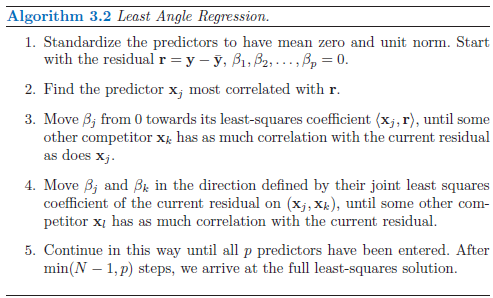
\includegraphics[width=0.7\textwidth]{Figures/LARAlgo}
\end{figure}
Let $\mathcal{A}_k$ be the active set at step $k$, $\beta_{\mathcal{A}_k}$ be the 
coefficient vector. There will be $k-1$ nonzero values and one zero. Let 
$r_k=y-X_{\mathcal{A}_k}\beta_{\mathcal{A}_k}$, then the direction for this step is
\begin{equation*}
\delta_k=(X_{\mathcal{A}_k}^TX_{\mathcal{A}_k})X_{\mathcal{A}_k}^Tr_k
\end{equation*}
Then coefficient profile evolves as
$\beta_{\mathcal{A}_k}(\alpha)=\beta_{\mathcal{A}_k}+\alpha\cdot \delta_k$. 
Let $u_k=X_{\mathcal{A}_k}\delta_k$, it makes the smallest and equal angle with each 
predictor in $\mathcal{A}_k$.  With LAR, we can know the step length at the beginning
of each step. 

%TODO:

\section{Methods of Derived Input Directions}
Large number of inputs with high correlation. This section describes how to linearly
combine $X_j$ to $Z_m$ used in regression. 
\subsection{Principal Components Regression}
Since $Z_m$ here are orthogonal, when regress $y$ for some $M<p$,
\begin{equation*}
\hat{y}_{(M)}^{\text{per}}=\bar{y}1+\sum_{m=1}^M\hat{\theta}_mz_m,\quad
\hat{\theta}_m=\frac{<z_m,y>}{<z_m,z_m>}
\end{equation*}
Since $z_m=Xv_m$, we have
\begin{equation*}
\hat{\beta}^{\text{per}}(M)=\sum_{m=1}^M\hat{\theta}_mv_m
\end{equation*}
Compared with Ridge, it discards the $p-M$ smallest eigenvalue components. 
 
\subsection{Partial Least Squares}
Assume $x_j$ is normalized(PLS and principal components regression are not
scale invariant). It begins by
\begin{equation*}
\hat{\varphi}_{1j}=<x_j,y>, \quad z_1=\sum_j\hat{\varphi}_{1j}x_j
\end{equation*}
Hence in the construction, inputs are weighted by the strength of their univariate 
effect on $y$. 
\begin{figure}[H]
    \centering
    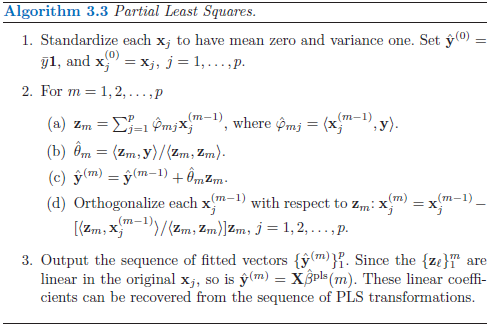
\includegraphics[width=0.7\textwidth]{Figures/PLSAlgo}
    \label{fig:}
\end{figure}
PLS seeks directions that have high variance and high correlation with the response. 
In particular, the $m$th principal component direction $v_m$ solves
\begin{equation*}
\max_\alpha Var(X\alpha) \quad\text{ subject to } 
||\alpha||=1,~\alpha^TSv_l=0,~l=1,2,...,m-1
\end{equation*}
where $S$ is the covariance matrix of $x_j$. $\alpha^TSv_l$ shows that $z_m=X_\alpha$
is uncorrelated with all $z_l=Xv_l$. 

On the other hand, the $m$th PLS direction solves
\begin{equation*}
\max_\alpha Corr^2(y,X\alpha)Var(X\alpha) \quad\text{ subject to } 
||\alpha||=1,~\alpha^TSv_l=0,~l=1,2,...,m-1
\end{equation*}
Further study shows that the variance part tends to dominant, so PLS behaves like 
Ridge/PCR. 

\section{A Comparison of the Selection and Shrinkage Methods}
\textbf{Ridge} shrinks all directions, but shrinks low-variance directions more. 

\textbf{PCR} leaves $M$ high-variance directions alone, and discards the rest. 

\textbf{PLS} also tends to shrink the low-variance
directions, but can actually inflate some of the higher variance directions.
This can make it a little unstable, and cause it to have slightly higher
prediction error compared to ridge regression.

\textbf{Conclusion}: PLS, PCR and ridge regression tend to behave similarly.
Ridge regression may be preferred because it shrinks smoothly, rather than
in discrete steps. Lasso falls somewhere between ridge regression and best
subset regression, and enjoys some of the properties of each.

\section{Multiple Outcome Shrinkage and Selection}
% TODO: 
\textbf{Simple Approach}: Apply a univariate technique individually to each outcome 
or simultaneously to all outcomes. 

Or we can exploit correlations in the different responses. 

\section{More on the Lasso and Related Path Algorithms}
% TODO: 


\section{Computational Considerations}
Least squares fitting is usually done via Cholesky decomposition of $X^TX$($p^e+Np^2/2$)
or QR decomposition($Np^2$). Lasso with LAR has the same order of computation. 